%===============================================================================
% $Id: ifacconf.tex 19 2011-10-27 09:32:13Z jpuente $  
% Template for IFAC meeting papers
% Copyright (c) 2007-2008 International Federation of Automatic Control
%===============================================================================
\documentclass{ifacconf}

\usepackage{graphicx}      % include this line if your document contains figures
\usepackage{natbib}        % required for bibliography
\usepackage{subfigure}
%===============================================================================
\begin{document}
\begin{frontmatter}

\title{DORIS - A MOBILE ROBOT FOR INSPECTION AND MONITORING OF
OFFSHORE FACILITIES\thanksref{footnoteinfo}} 
% Title, preferably not more than 10 words.

\thanks[footnoteinfo]{This work is supported primarily by Petrobras S.A. and
Statoil Brazil Oil \& Gas Ltda under contract COPPETEC 0050.0079406.12.9
(ANP-Brazil R \& D Program), and in part by the Brazilian research agencies CNPq
and FAPERJ}

\author[First]{First A. Author} 
\author[Second]{Second B. Author, Jr.} 
\author[Third]{Third C. Author}
\author[Forth]{Forth D. Author}

\address[First]{Research and Development Center, Petrobras/CENPES, Rio de
Janeiro, Brazil} 
\address[Second]{Mathematical Sciences and Technology Department, Norwegian
University of Life Sciences, Oslo, Norwegian }
\address[Third]{Electrical
Engineering Department, COPPE UFRJ, Rio de Janeiro, Brazil, (e-mail: )}
\address[Forth]{TPD RD New Development Solutions, Statoil ASA}

\begin{abstract}                % Abstract of not more than 250 words.
DORIS is a research project which endeavors to design and implement a mobile
robot for remote supervision, diagnosis, and data acquisition on offshore
facilities. The proposed system is composed of a railguided robot capable of
carrying different sensors through the inspected area. This paper presents a
general overview of the robot and a description of the developed software
architecture, embedded electronics and power supply system. Initial results
with teleoperational navigation validate the concepts considered so far and
rise several challenges in the three fields.
\end{abstract}

\begin{keyword}
Mobile robots; Field robotics; Decurity and safety of HMS.
\end{keyword}

\end{frontmatter}
%===============================================================================

\section{Introduction}
Safety and efficient operation are imperative factors to offshore production
sites and a main concern to all Oil \& Gas companies. A promising solution to
improve both safety and efficiency is to increase the level of automation on
the platforms by introducing robotic systems.

During the last decade, several Oil \& Gas companies, research groups, and
academic communities have shown an increasing interest in the use of robots for
operation on offshore facilities.  

Recent studies project a substantial decrease in the level of human operation
and an increase in automation on future offshore oil fields
~\cite{skourup2009robotized}.The studies also point out the potential increase
in efficiency and productivity with robot operators, besides the improvement of
Health, Safety, and Environment (HSE) conditions, as robots can replace humans
in tasks performed in unhealthy, hazardous, and confined areas ~\cite{pal}. 
In~\cite{abb}, it is considered the use of robots in Oil \& Gas facilities in
operations that require both high precision and strength, regardless of weather conditions.

In the specific case of Brazil, the Oil \& Gas industry is growing at a high
pace, mainly due to the recent discoveries of big oil fields in the pre-salt
layer off the Brazilian coast. These oil reservoirs are located farther than
300 km from the shore and at depths of 5000 to 7000 km. These factors,
especially the large distances, motivate the development of an offshore
production system with a high degree of automation based on advanced robotics
systems.

Among the research groups interested in offshore robotics, \emph{Fraunhofer
IPA} is pioneer in proposing and demonstrating the applicability of mobile
robots for offshore inspection and maintenance tasks \emph{in
loco} ~\cite{mimroex2}. One example is MIMROex ~\cite{mimroex}, capable of
navigating safely, building maps, and executing inspection tasks autonomously
throughout the topside of platforms.

Another robotic device applied in offshore environments is Sensabot
~\cite{sensabot}, capable of safely inspect and monitor hazardous and remote
production facilities. The robot can sustain high temperatures, is able to
reach areas with difficult access, and is certified to operate in explosive and
toxic environments.

SINTEF-ICT is another group interested in manipulators applied to the oil and
gas industry. Inspection and maintenance operations in a simulated production
process are performed by the cooperation of a gantry-mounted manipulator and a
floor-mounted robot ~\cite{kyrkjebo2009robotic}.

In this paper, we describe the DORIS project, which aims to develop a mobile
robot to perform monitoring, inspection, and simple intervention tasks in an
offshore platform. To this end, the system must be able to move throughout the
monitored environment carrying different sensors, analyzing sensor data
\emph{in loco} or storing it for a posterior analysis, and interpreting the
results. The sensors can identify abnormalities such as intruders in restricted
areas, abandoned objects, smoke, fire, and liquid and gas leakages.
Furthermore, the robot is able to make machinery diagnosis, read instruments,
and perform interventions on valves and other equipment using an embedded manipulator.

The paper is organized as follows: a general overview of the robot and its main
challenges are presented in Section \ref{sec:general_overview}, detailed
descriptions of the software architecture, embedded electronics and power supply
system are taken in Sections \ref{sec:software_overview},
\ref{sec:electronics_overview} and \ref{sec:powersupply_overview} respectively.
In Section \ref{sec:results}, preliminary results are shown, and concluding
remarks are drawn in Section \ref{sec:conclusions}. 

% Please stick to the format defined by the \texttt{ifacconf} class, and
% do not change the margins or the general layout of the paper. It
% is especially important that you do not put any running header/footer
% or page number in the submitted paper.\footnote{
% This is the default for the provided class file.}
% Use \emph{italics} for emphasis; do not underline.
% 
% Page limits may vary from conference to conference. Please observe the 
% page limits of the event for which your paper is intended.

\section{General Overview}\label{sec:general_overview}

The proposed system is composed of a robot with cameras, microphones, gas,
vibration and temperature sensors, and a manipulator arm. The robotic device is
guided by a rail and both the robot and the rail follows a modularity concept.
Additional robot modules can be annexed to include other sensors, and the rail
track can be modified by adding or replacing rail segments, thus enabling
operation in different areas of the platform.% Robot modules are organized by
% functionality, for example, traction and sensing modules.

The robot will be controlled autonomously or by teleoperation. Task managing
can be either in automatic (programmed using a mission interface) or manual
mode (real-time remote operation). The teleoperation and monitoring
capabilities guarantee online access to the embedded sensors, providing
information about the surrounding environment and the robot operating
conditions with real-time processing. Figure~\ref{fig:DORIS-overview}
illustrates the operation in a production plant.

%\begin{figure} [!h]
%    \begin{center}
%    \includegraphics[width=8.8cm]{figs/DORIS_overview.jpg}  % width is 8.4 cm.
%    \caption{Illustration of the DORIS robot operating in a platform topside environment}
%    \label{fig:DORIS-overview}
%    \end{center}
%\end{figure}

\begin{figure}[ht]
\centering
\subfigure[Robot's operational scenario in a production plant]{%
    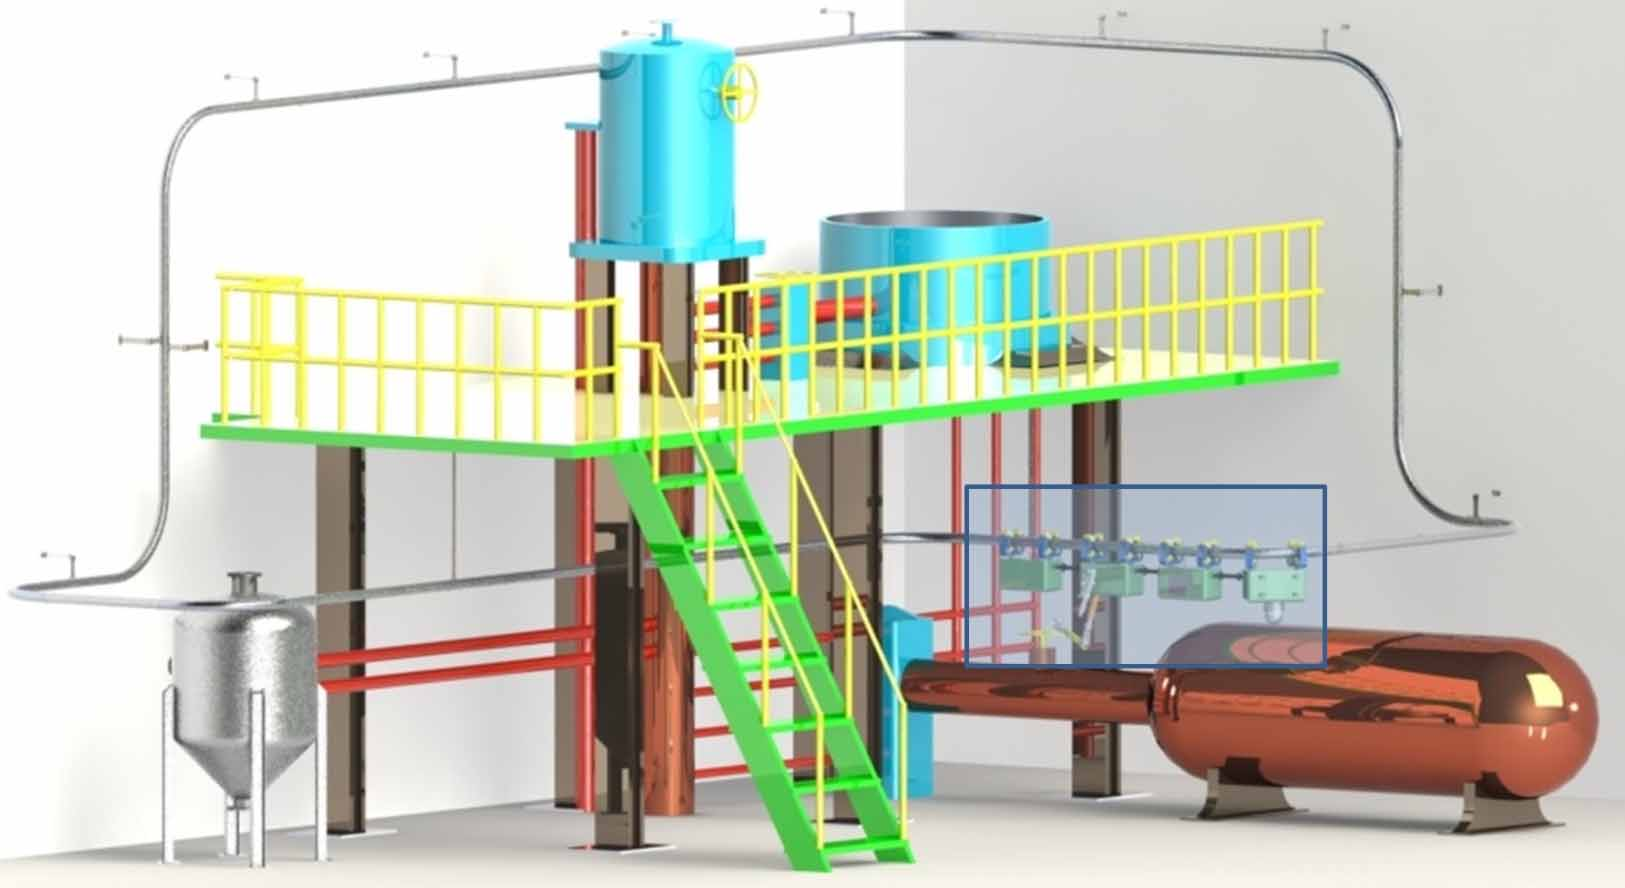
\includegraphics[width=8.4cm]{figs/cenario1.jpg}  % width is 7.6 cm.
    \label{fig:cenario1}} 
\subfigure[Detailed zoom of the robot]{%
    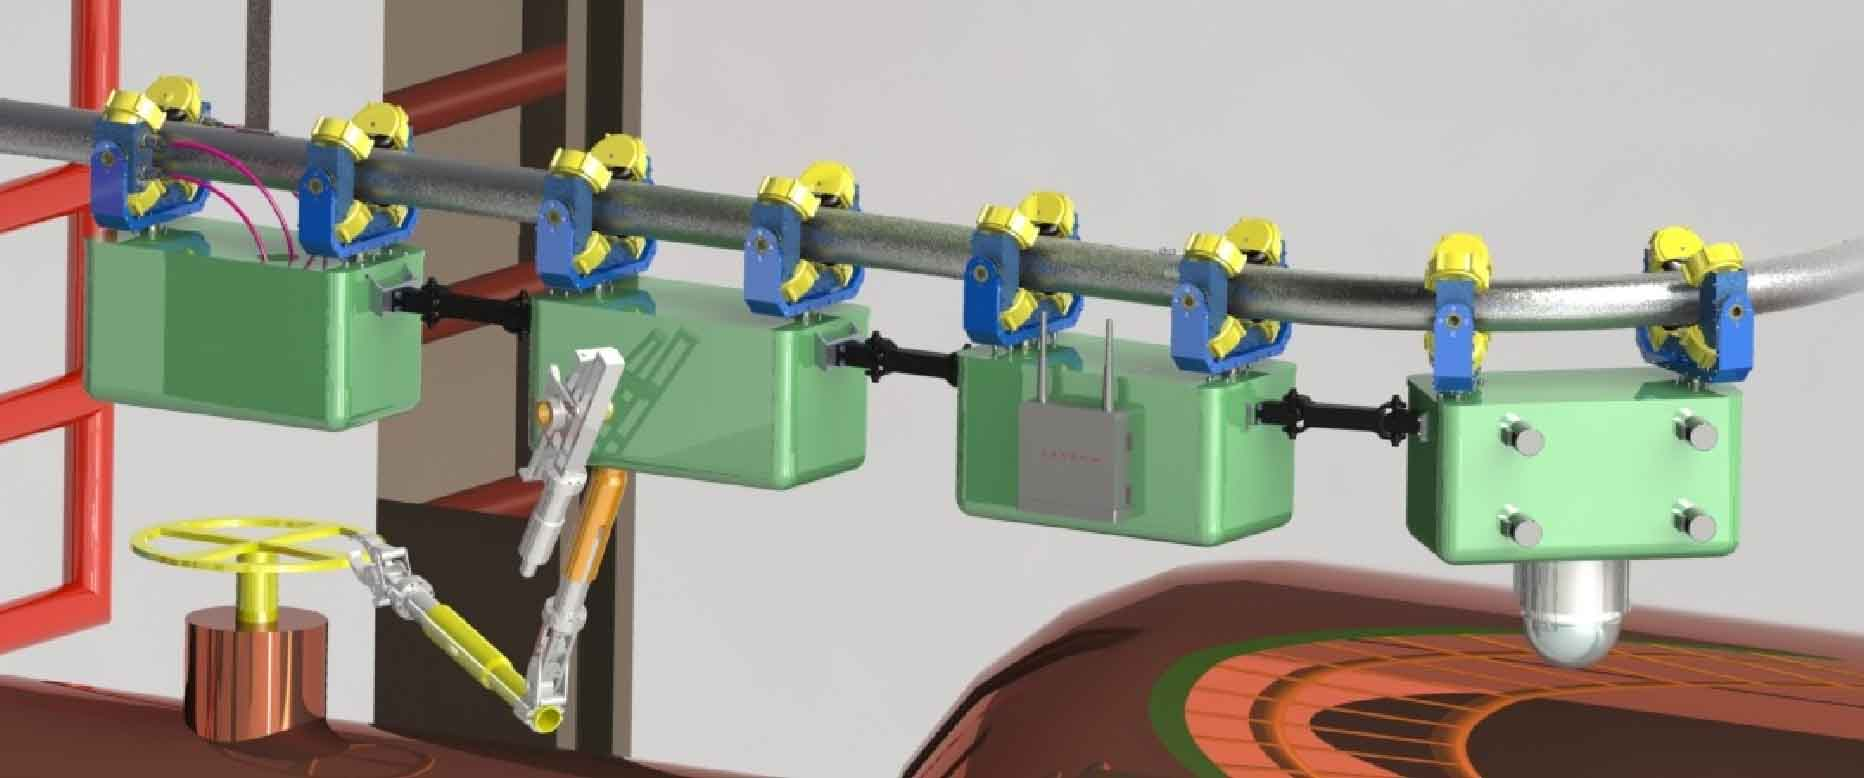
\includegraphics[width=8.4cm]{figs/zoom.jpg}  % width is 7.6 cm.
    \label{fig:zoom}}\vspace{-.1cm}
\caption{Illustration of the DORIS robot operating in a production plant.}\vspace{-0.25cm}
\label{fig:DORIS-overview}
\end{figure}

The DORIS project can be divided into five subsystems: electronics, power
supply, software, mechanics and signal processing.

%-------------------------------------------------------------------------------------------------------------------------
%ELECTRONICS
%-------------------------------------------------------------------------------------------------------------------------
The electronics subsystem is responsible for providing embedded computational
support for the robot control, signal processing, task managing, and local and
remote communication. The device motion is controlled through drivers that can
receive position, velocity, or current setpoints. The embedded electronics has
two printed circuit boards for the vehicle support system: energy distribution
and monitoring, basic failure detection, emergency handling and devices'
control.
% (EPOS from Maxon Motors)

%Concerning robustness and safety required to operate in harsh environments, the robot  must be sealed against water and ingress of objects, resistant to a wide temperature range, protected from impact and vibration, electrically protected to avoid explosion by ignition, and equipped with a monitoring system.%protected 2x?

%-------------------------------------------------------------------------------------------------------------------------
%POWER SUPPLY
%-------------------------------------------------------------------------------------------------------------------------
The power supply system uses military-class lithium-ion batteries, which have
small size and high energy capacity. In the first prototype of DORIS, four
batteries are used to power the motors and two to power the other electronics
components. 

%Considering the requirements to operate in harsh environments and classified areas,

%-------------------------------------------------------------------------------------------------------------------------
%SOFTWARE
%-------------------------------------------------------------------------------------------------------------------------
The main objective of the software subsystem is to allow the implementation of
high- and low-level control of the robot. The tools used to develop DORIS
software architecture must consider two important factors: they have to be
commercially available, and provide modular functionalities. These requirements
led to the adoption of Qt as the graphical interface framework ~\cite{qt},
Robot Operating System (ROS) as the communication middleware ~\cite{ros}, and
Ubuntu as the operating system.

%Robots may be very complex, so it is important to divide this complexity into smaller, independent parts.

The software provides autonomous control (programmed tasks) and remote control
through a Graphical User Interface (GUI) in the Host Control Base (HCB)
computer. The HCB is composed of a set of processes running in parallel
denominated ROS nodes, which can communicate with each other. To deal with this
environment, a new software architecture called Robot Package Software is
proposed, dividing the software into tools (graphical windows) and components
(processing and communication unities), and grouping them into a dynamic
library. %A DORIS Package is developed as a library containing a list of components and tools for the DORIS robot.

%Firstly, the robot needs to perform the task it is set to do and do so in the safest and most efficient way. This may include the control of the robot and machine learning algorithms. The software also needs to be suited for low-level control of the various components when this is not embedded.

%-------------------------------------------------------------------------------------------------------------------------
%Mechanics
%-------------------------------------------------------------------------------------------------------------------------
The mechanical project designs the rail, the
traction and passive modules, and the joints used to couple them. The design
allows the robot to move smoothly in a 3D space and makes full stop anywhere
on the rail. Considering the severe corrosion and weather conditions in
offshore environments, the choice of materials are imperative to the success of
the project and certified solutions must be considered.

The robot is composed of two modules at its default configuration, but it is
conceived so that other modules can be added. The total weight of this
configuration is estimated at 50 kg and we expect to have a maximum speed of
1m/s.

The design incorporates the use of gimbals with wheels as guides for
the module on the rail \cite{cba}. In the new configuration, the motors are
fixed on the gimbal and transmit its torque to the wheels via spur gears. The use of gimbals
is an proper choice concerning stability, guidance, and support. Furthermore,
it is possible to have a smooth vertical motion applying radial forces by the
clamping mechanism.

%-------------------------------------------------------------------------------------------------------------------------
%DSP
%-------------------------------------------------------------------------------------------------------------------------


%-------------------------------------------------------------------------------------------------------------------------
%OTHER CHALLENGES
%-------------------------------------------------------------------------------------------------------------------------
Considering the robot functionalities and the aggressive offshore environment,
several challenges should be addressed. Temperatures in offshore facilities can
vary between $-30^{\circ}$C to $50^{\circ}$C, relative humidity can reach
100\%, and there may be splash water, salty air, storms, and high extensive
corrosion ~\cite{graf2007mobile}. 

Concerning robustness and safety required to operate in classified areas, the
robot must be sealed against water and objects, resistant to a wide temperature
range, protected from impact and vibration, electrically shielded to avoid
explosion by ignition, and equipped with a monitoring system.

%{\color{red}Moreover, the robot parts must have special enclosures to turn it explosion-proof and allow operation in classified areas.}

Another challenge is that the embedded computers must run heavy signal
processing algorithms, requiring high computational power. However, the power
supply subsystem must efficiently provide power and maintain a low level of
power consumption.

Further complications arise because the system is designed to move in confined
areas and have efficient wireless communication with operators, providing
online information of sensors data. Finally, the robot must have a modular and
flexible design, employing plug and play extensions.%, which represents an
% additional complication.%challenge?




\section{Embedded Electonics}\label{sec:electronics_overview}

\section{Power supply system}\label{sec:powersupply_overview}
This part of the robot is responsible for reliable, safe and efficient delivery
of electric energy on each equipment inside DORIS. The power supply of choice
is a high density energy level military lithium ion battery model, shown in 
figure~\ref{fig:bat}, which comes with intrinsically safety circuit in order to
avoid possible short-circuits or heat problem, disabling the battery itself in
cases of safety risks. The model currently in use has a 10Ah capacity, where
four units are located on each module, weighting 1.4Kg each.

\begin{figure}[ht]
\centering
%\subfigure[Robot's operational scenario in a production plant]{%
    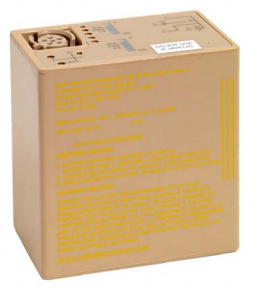
\includegraphics[width=0.5\columnwidth]{figs/bateria.png}  % width is 7.6 cm.
    \label{fig:bat}
\caption{Military Li-on Battery Model.}\vspace{-0.25cm}
%\label{fig:DORIS-overview}
\end{figure}

As Verma et al. (2004) highlight, robots often operate in environments where
human intervention is expensive, slow, unreliable, or impossible. It is
therefore essential to monitor their behavior so that faults may be addressed
before they result in catastrophic failures. The power management interface is
implemented through System Management Bus (SMBus) connections with the robot
microprocessor, allowing the electronics to receive all possible information
about each battery condition. As the robot is intended to work inside offshore
platforms, which are hazardous areas, one must always consider the classified
are zone with the highest restrictions that the robot will potentially move
into.

In order to avoid avoid EMI and conductive noise interference, the project
currently works with two separate power buses, each of these built using two
24Vdc batteries connected in parallel, being able to deliver a capacity of
20Ah. One bus is dedicated to power the motors and the other, to power all
electronic equipment. Also, DC/DC converter shown in figure~\ref{fig:conv} are
being used to create different voltage levels (12Vdc and 5Vdc) and also to
ensure a stable power source (even for 24Vdc components). Also, diodes are
being used in order to avoid back-flow current.

\begin{figure}[ht]
\centering
%\subfigure[Robot's operational scenario in a production plant]{%
    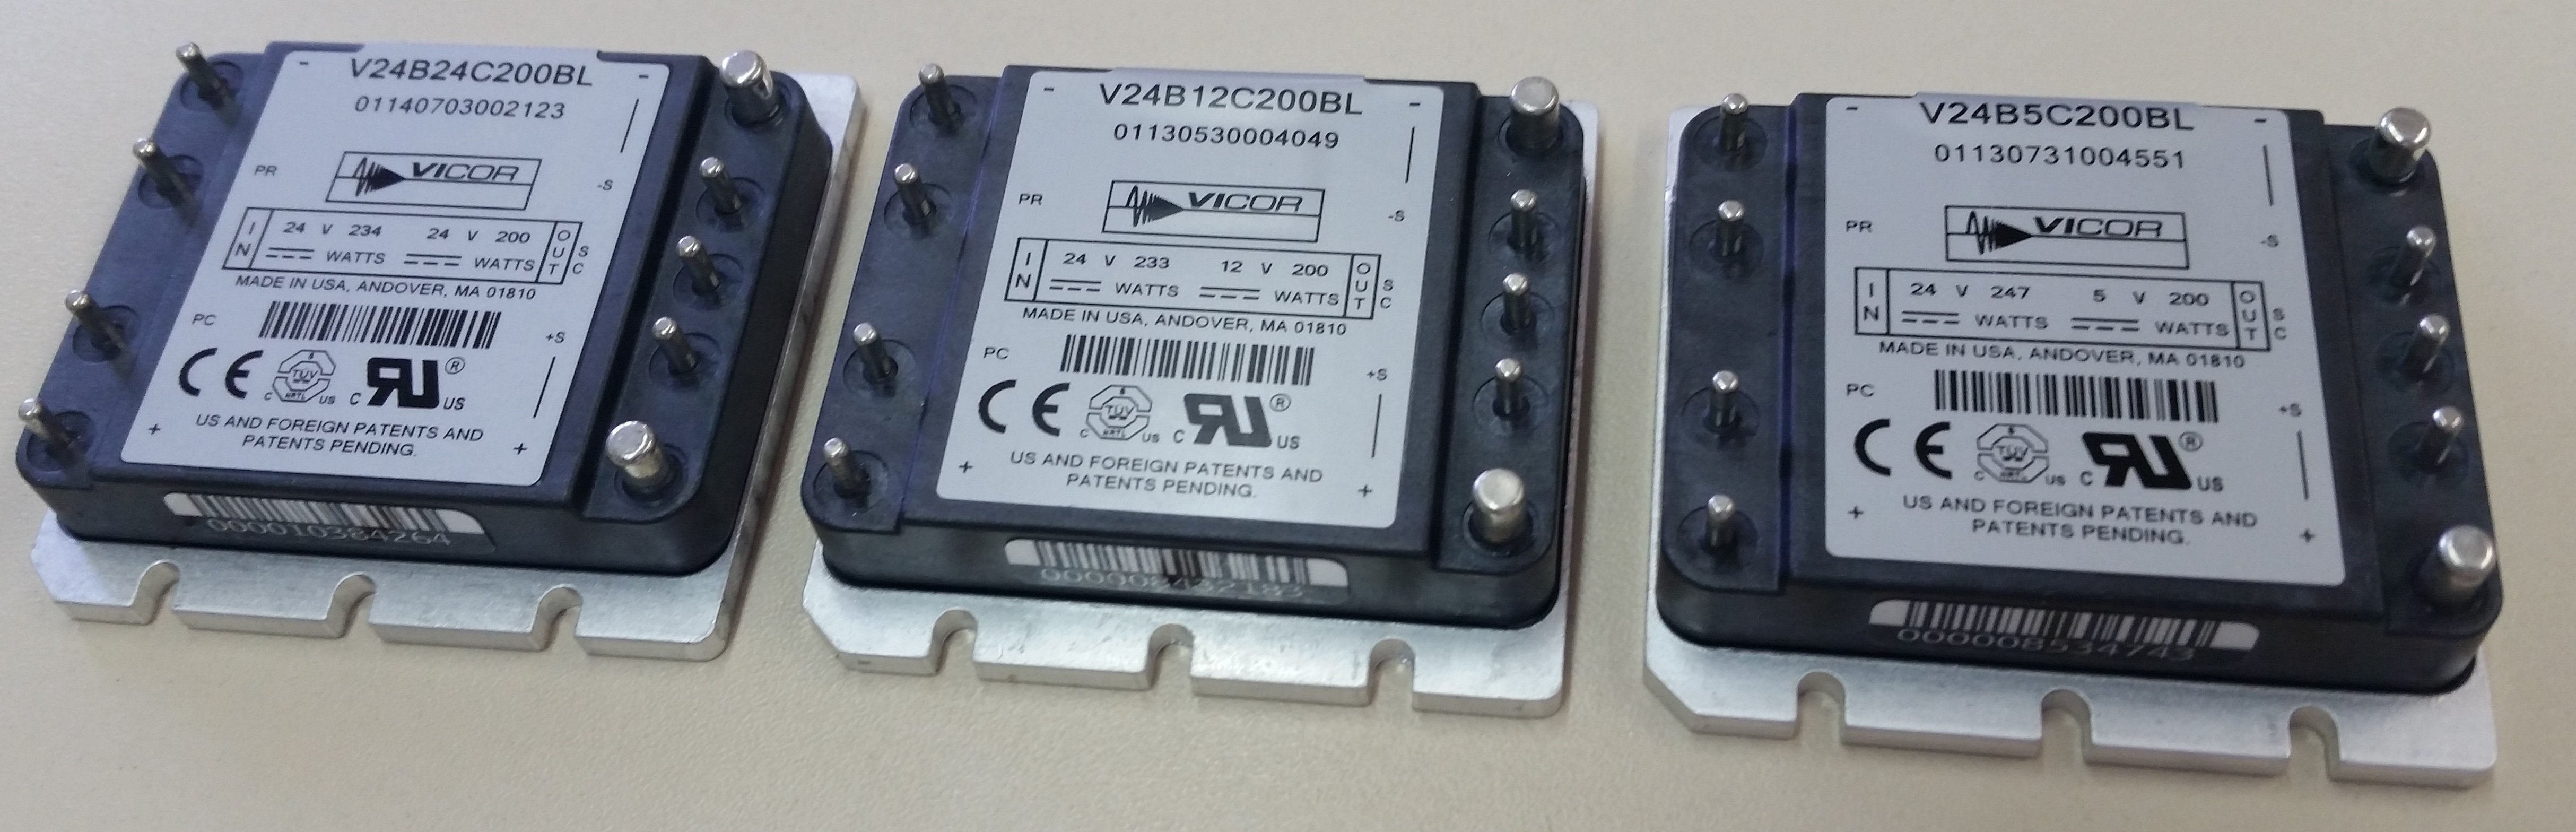
\includegraphics[width=1\columnwidth]{figs/Conversores.jpg}  % width is 7.6 cm.
    \label{fig:conv}
\caption{DC/DC Converters for 24Vdc input and 24Vdc, 12Vdc and 5Vdc outputs.}\vspace{-0.25cm}
%\label{fig:DORIS-overview}
\end{figure}

Also, diodes are being used in order to avoid back-flow current, fuses are
protecting the system from undesired peaks just after each DC/DC converter and
buttons allow the each power bus to be separately turned on/off.

For the power buses connections it is being used a stub block, like the one
shown in figure~\ref{fig:bar}, to make all connection between batteries and the
system, creating the the parallel connection for each bus.

\begin{figure}[ht]
\centering
%\subfigure[Robot's operational scenario in a production plant]{%
    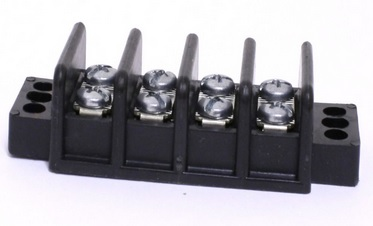
\includegraphics[width=0.6\columnwidth]{figs/bar2.jpg}  % width is 7.6 cm.
    \label{fig:bar}
\caption{Stud Bar for Parallel Connnection on the Power Buses.}\vspace{-0.25cm}
%\label{fig:DORIS-overview}
\end{figure}

The current architecture of the power supply embedded on this project is
illustrated on figure~\ref{fig:DiagramaSAM}. The electronics power bus in
currently installed using 14AWG wires for up to 15A of nominal current and the
motors power bus is currently installed using 12AWG wires for up to 21A of
nominal current.

\begin{figure}[ht]
\centering
%\subfigure[Robot's operational scenario in a production plant]{%
    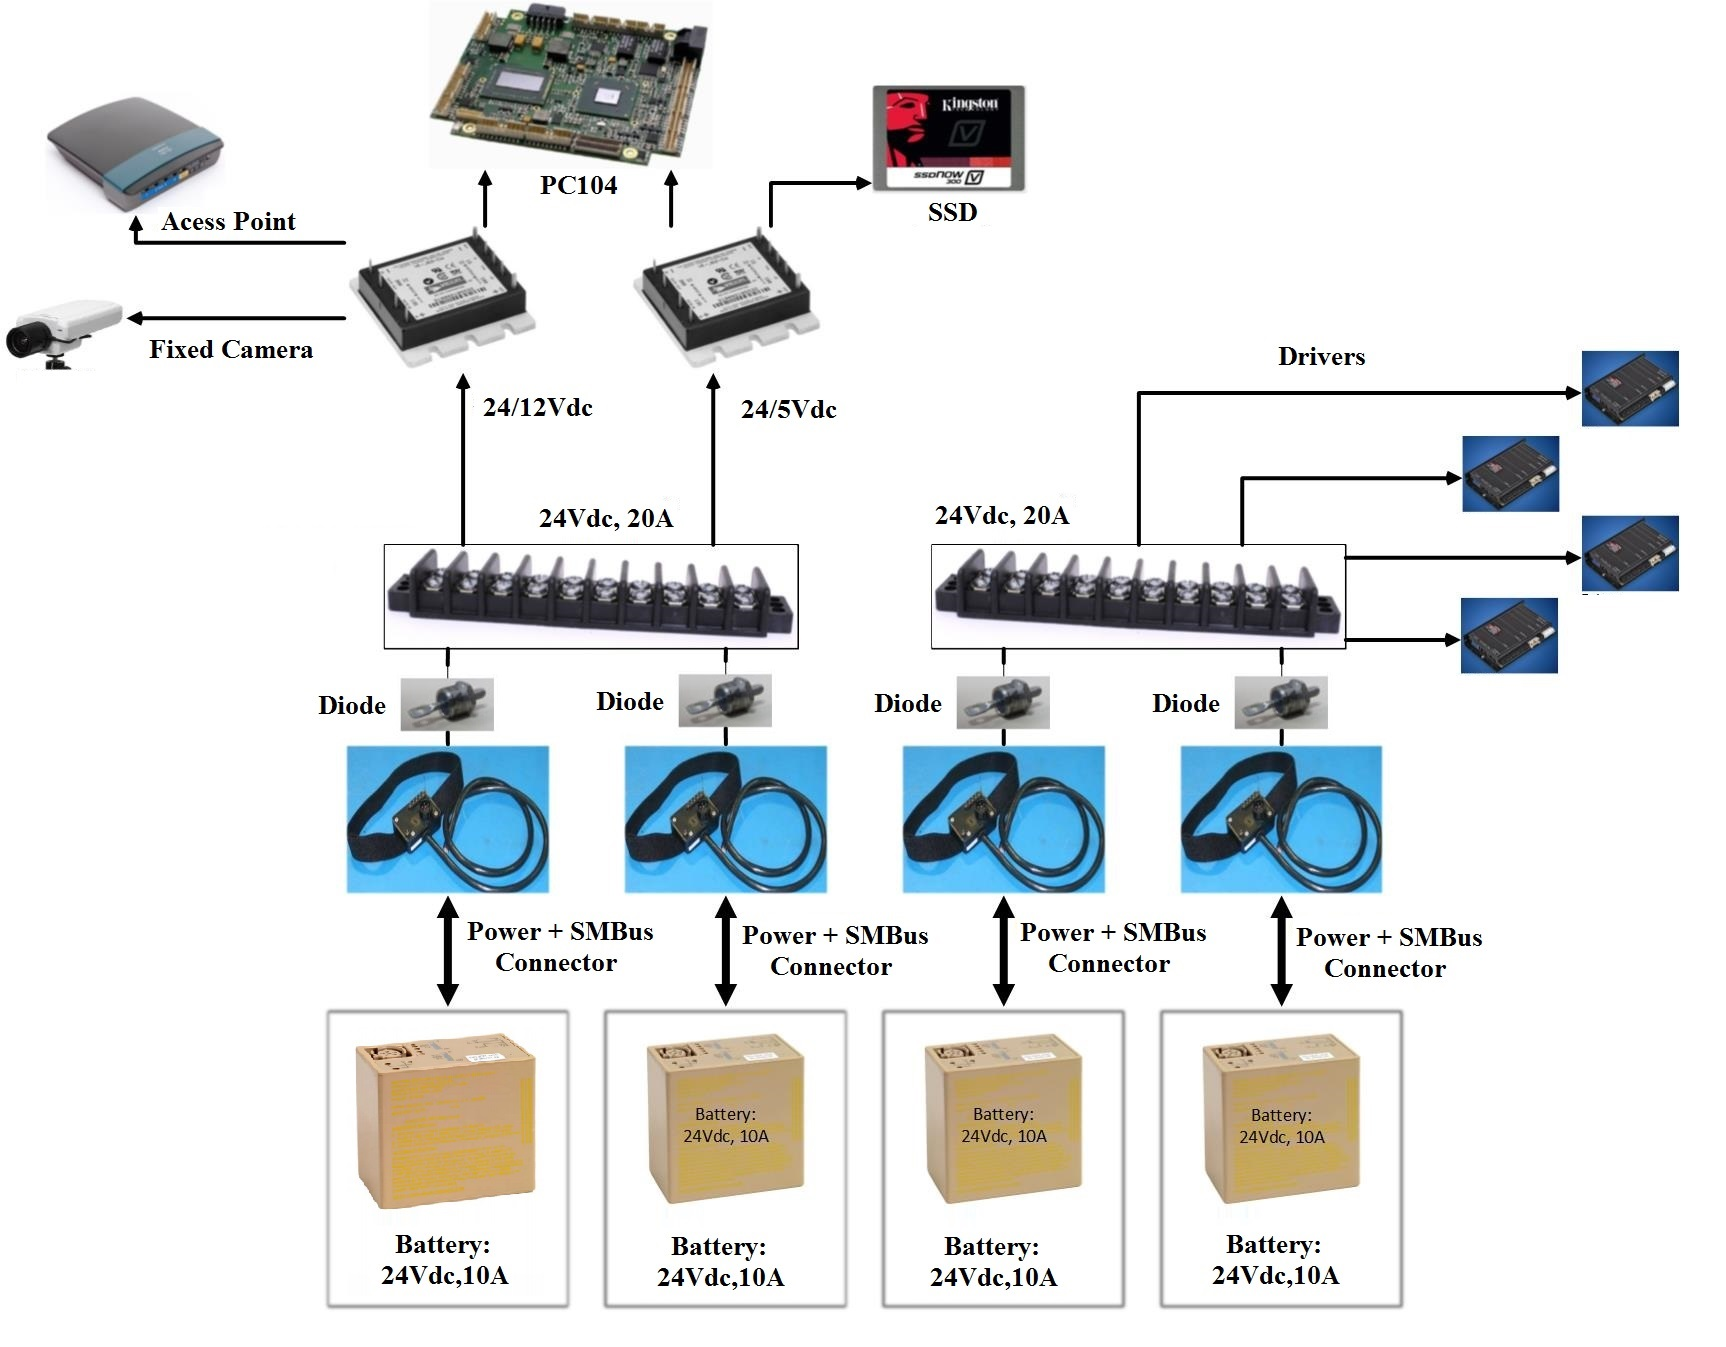
\includegraphics[angle=90,width=1\columnwidth]{figs/DiagramaSAM.jpg}  % width is 7.6 cm.
    \label{fig:DiagramaSAM}
\caption{Power Supply Architecture.}\vspace{-0.25cm}
%\label{fig:DORIS-overview}
\end{figure}

Considering this, new challenges came up in order to improve the features of
the system.

\subsection{Achievements}

To achieve a high level of robustness, two approaches are being developed in
order to switch any battery between any of the power buses, as shown in
figure~\ref{fig:DORIS-PCBs}: a printed circuit board, PCB, for (a) manual
switching option will allow the operator to manually connect each battery into
one of the buses before turning on the robot or (b) an automatic switching PCB
option, where solid state relays commanded by the BMS system will allow the
on-line switching of each battery if by any reason the operator thinks it would
be best to give more power to a specific bus or even in emergency cases where a
battery may be taken from a bus to compensate, for instance, a battery loss on
the other bus.

\begin{figure}[ht]
\centering
\subfigure[Manual Switch PCB]{%
    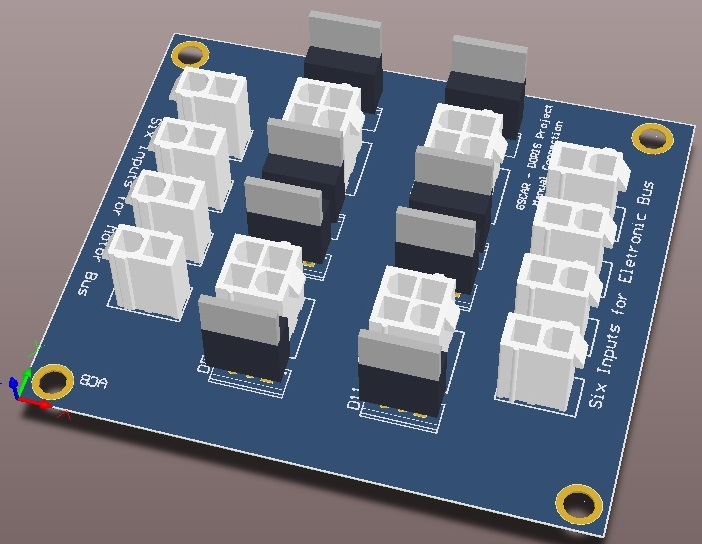
\includegraphics[width=0.8\columnwidth]{figs/manual4.jpg}  % width is 7.6 cm.
    \label{fig:cenario1}}
\subfigure[Automatic Switch PCB]{%
    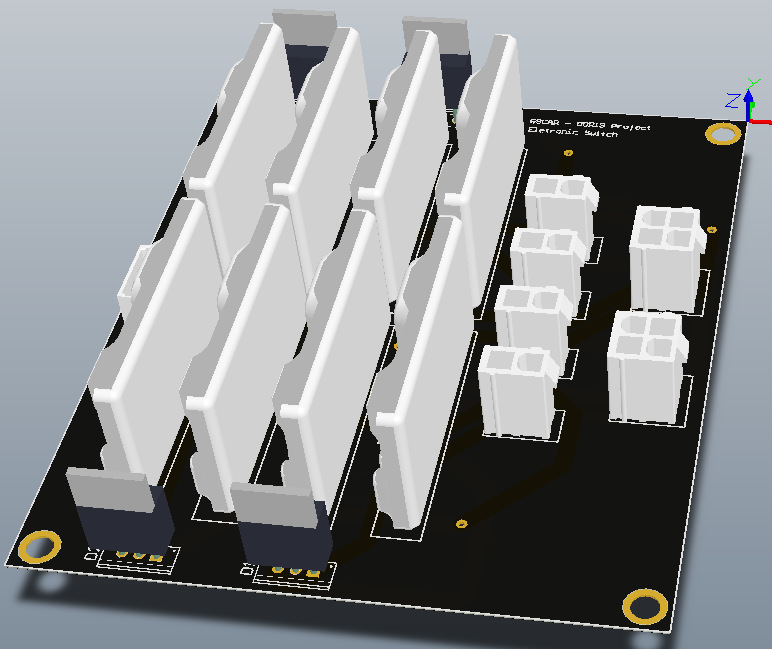
\includegraphics[width=0.8\columnwidth]{figs/Top2.png}  % width is 7.6 cm.
    \label{fig:zoom}}\vspace{-.1cm}
\caption{Illustration of the Power Bus Switching Boards Options.}\vspace{-0.25cm}
\label{fig:DORIS-PCBs}
\end{figure}

An last issue observed on this project is the fact that when going downwards
the motor generates energy. Depending on the height of the fall and the
velocity of DORIS, the energy created may reach voltage levels that cause the
drivers to stop. Because of this, the group is working on ways to measure de
energy level created and decide if it would be worth to store this energy or if
it would be better to simply discard it by using a shunt regulator.

Thus, DORIS is equipped with a power supply system with an improved robustness
level when compared with other robotic systems and it also has a considerable
light weight, high energy density and increased safety properties.


\section{Software architecture}\label{sec:software_overview}

\section{Conclusion}\label{sec:conclusions}
 

\begin{ack}
Place acknowledgments here.
\end{ack}

\bibliography{ifacconf}             % bib file to produce the bibliography
                                                     % with bibtex (preferred)
                                                   
%\begin{thebibliography}{xx}  % you can also add the bibliography by hand

%\bibitem[Able(1956)]{Abl:56}
%B.C. Able.
%\newblock Nucleic acid content of microscope.
%\newblock \emph{Nature}, 135:\penalty0 7--9, 1956.

%\bibitem[Able et~al.(1954)Able, Tagg, and Rush]{AbTaRu:54}
%B.C. Able, R.A. Tagg, and M.~Rush.
%\newblock Enzyme-catalyzed cellular transanimations.
%\newblock In A.F. Round, editor, \emph{Advances in Enzymology}, volume~2, pages
%  125--247. Academic Press, New York, 3rd edition, 1954.

%\bibitem[Keohane(1958)]{Keo:58}
%R.~Keohane.
%\newblock \emph{Power and Interdependence: World Politics in Transitions}.
%\newblock Little, Brown \& Co., Boston, 1958.

%\bibitem[Powers(1985)]{Pow:85}
%T.~Powers.
%\newblock Is there a way out?
%\newblock \emph{Harpers}, pages 35--47, June 1985.

%\bibitem[Soukhanov(1992)]{Heritage:92}
%A.~H. Soukhanov, editor.
%\newblock \emph{{The American Heritage. Dictionary of the American Language}}.
%\newblock Houghton Mifflin Company, 1992.

%\end{thebibliography}

\appendix
\section{A summary of Latin grammar}    % Each appendix must have a short title.
\section{Some Latin vocabulary}              % Sections and subsections are supported  
                                                                         % in the appendices.
\end{document}
